\documentclass{article}
\usepackage{graphicx}
\usepackage{wrapfig}
\usepackage{fullpage}

\begin{document}


\title{Haalbaarheidsstudie IN2710-D/TI2710-D}
\author{\begin{tabular}{l l}
Jeroen Bareman & 4035186\\
Roelof Sol & 4012194\\
Mick van Gelderen & 4091566\\
Luyt Visser & 4016603\\
Jelle Licht & 4106946\end{tabular}\\
Groep 6}
\maketitle
\newpage

\section{Doelen}
Het doel voor dit project is een robot programmeren die zelfstandig de uitgang van een doolhof kan vinden. Dit doolhof moet voldoen aan de gestelde omgevingseisen toegelicht in kop 2.
Om het projectdoel te bereiken zal de robot de uitgang moeten kunnen vinden door rond te rijden zonder te botsen. Om de robot te laten bewegen moet deze om zijn as kunnen draaien en rechtdoor kunnen rijden. 
Om ervoor te zorgen dat de robot niet botst zal deze de obstakels en muren moeten ontwijken. Deze kan hij waarnemen met zijn sensoren.

\section{Beschikbaar materiaal}
De basis is een chassis met twee rupsbanden met een lengte van 20cm en een breedte van 13 cm. De diagonaal van de tank is ~24 cm lang. Deze worden elk door een aparte motor aangedreven zodat het mogelijk is om rond te draaien. In de chassis zit een batterij en een processing board met daarop een StrongARM SA-1100 processor die de mogelijkheid heeft om Linux kernel 2.6 te draaien. Deze kernel zal de andere componenten van de robot
aansturen. Om met de kernel te communiceren en er eigen software op te zetten, wordt een seriële verbinding gebruikt. De randapparatuur die de processor zal gebruiken bestaat uit:

\begin{itemize}
\item{Een “SN754410 Quadruple Half-H Driver” die twee motoren bevat, die elk apart de standen uit, vooruit , achteruit kunnen aannemen. De afzonderlijke motoren worden aangestuurd mbv 3 GPIO pinnen.}
\item{Vier “SRF02 Ultrasonic range finder” die afstanden kunnen bepalen om de 66ms met een minimale afstand tussen de 11 en 16 cm, afhankelijk van de temperatuur en andere factoren. Twee zijn er gemonteerd aan de voorkant en twee aan de zijkant. Deze sensoren zijn uit te lezen door gebruik te maken van het I²C protecol.}
\item{Een “CMPS03 Robot Compass Module” die accuraat genoeg is om het magnetisch veld van de aarde te detecteren en een getal terug geeft tussen de 0 en 3599, waarbij tien eenheden staan voor 1$^\circ$. Communicatie met de kompasmodule verloopt via het I2C protocol.}
\item{Twee knoppen die gebruikt kunnen worden om input te geven.}
\item{Twee LEDs die gebruikt kunnen worden om feedback te geven.}
\end{itemize}

\section{Omgevingseisen}
\begin{wrapfigure}{r}{0.35\textwidth}
  \vspace{-10pt}
  \begin{center}
    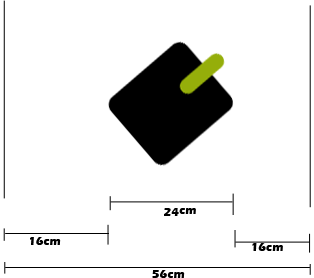
\includegraphics[width=0.34\textwidth]{tank_kunst.png}
  \end{center}
  \vspace{-10pt}
  \caption{(a)maze(ing) dimensions}
  \vspace{-50pt}
\end{wrapfigure}
De robot moet de ruimte hebben om te kunnen draaien in het doolhof. 
Aangezien voor de ultrasoon sensoren een minimale afstand tot de muur van ~16 cm geld, kan je zeggen dat de tank minimaal
2 maal afstand tot muur + diagonaal tank = $2 * 16 cm + 24 cm= 56 cm$ nodig heeft om overal goed te kunnen draaien. Als dit niet het geval
is kan het voor komen dat de robot tijdens het draaien vast komt te zitten, aangezien de sensoren op kleinere afstanden niet werken.

De robot moet over alle paden van het doolhof kunnen rijden. Zo moet er genoeg wrijving
met de ondergrond zijn en moet de robot door alle zichtbare gangen kunnen rijden.
Het doolhof moet op te lossen zijn, dwz dat het doolhof een uitgang moet hebben.

\newpage
\section{Invloed limited resources op doelen}
De beschikbare hardware limiteert samen met de omgeving de mogelijke methoden die
gebruikt kunnen worden om het doel te bereiken.
De meest voor de hand liggende beperkingen zijn de processorkracht en de hoeveelheid
geheugen. Dit heeft directe consequenties voor de algoritmen die gekozen kunnen worden. De keuze van het algoritme is echter niet op basis van deze beperkingen gemaakt. 

De sensoren die op de robot zitten zijn van gemiddelde kwaliteit. Ze hebben bijna allemaal
een verschillende standaard afwijking en moeten om geschikte metingen te krijgen
afzonderlijk gekalibreerd worden.

De software wordt ontwikkeld voor een embedded systeem. Dit betekent dat testen en
debuggen lastiger is dan dat het zou zijn op een pc. De input hangt af van programma
variabelen en metingen van sensoren. Om de programma variabelen te veranderen moet het
programma opnieuw naar de robot geupload worden wat meer tijd kost dan het alleen
compilen. De informatie die de sensoren leveren kan veranderd worden door de omgeving
te veranderen of door met het programma neppe waarden te geven. De output bekijken is
ook lastiger omdat, buiten de 2 leds om, de robot hiervoor verbonden moet worden met de
computer. De robot moet een bepaald gedrag gaan vertonen. Het kost veel tijd om te
observeren of de robot het gewenste gedrag vertoont waardoor er een aanzienlijke
hoeveelheid tijd nodig is voor het testen.

Naast de hierboven genoemde limiterende factoren die te maken hebben met de robot zelf,
zijn er ook beperkingen die de omgeving waarin de robot moet functioneren met zich mee
neemt. De gangen en kruispunten in het doolhof hebben een bepaalde breedte waar
rekening mee gehouden moet worden. Dit betekent dat de sensoren belangrijk zijn en dat de
signalen ervan zo nauwkeurig mogelijk uitgelezen moeten worden. Achteruit rijden om te
keren is lastig.

\section{Aanbevelingen}
Zoals in kop 4. naar voren komt is de robot is een embedded system met weinig resources.
Bij de opdracht wordt de tank in het doolhof neergezet, de enige uitweg is de uigang.
Het Pledge algoritme is in deze situatie dan ook uitermate geschikt. Wall hugging is ook goed te doen maar minder verschillende soorten doolhoven aan. Een aantal andere algoritmen gaan er van uit dat ze de kaart van het doolhof tot hun beschikking hebben. Pledge kan daarentegen on the fly beslissingen maken. Het voordeel van dit
algoritme is dat de uitgang in een eerlijk doolhof uiteindelijk altijd wordt gevonden zonder
dat er een interne representatie van zijn omgeving hoeft te worden bijgehouden. Het nadeel is dat Pledge niet werkt
bij doolhoven met zowel een externe ingang als uitgang. 

Als er bij de projectleden onderling vragen zijn, blijf dan niet zitten maar maak gebruik van
de projectgroep. Een goeie methode is om vragen gelijk op de mail te zetten zodat alle
projectleden hier gelijk over na kunnen denken of op kunnen reageren. Als deze problemen
dan tijdens een vergadering worden besproken weet iedereen al waar het over gaat, dit
scheelt tijd en zo kunnen we adequaat en efficiënt werken.

\end{document}
